\begin{figure}[t!]
% \vspace{-15pt}
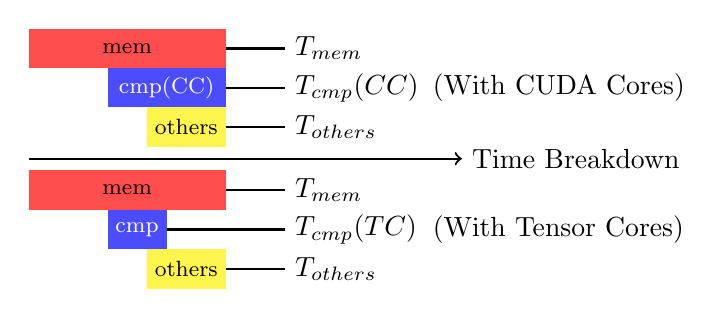
\begin{tikzpicture}[scale=0.5, every node/.style={scale=1}]
    % Timeline axis
    \draw[->, thick] (0,0) -- (11,0) node[right] {\textbf\footnotesize{Time Breakdown}};
    % Memory and Compute bars
    \fill[red!70] (0,2.3) rectangle (5,3.3) node[pos=.5,black] {\footnotesize{mem}};
    \fill[blue!70] (2,1.3) rectangle (5,2.3) node[pos=.5,white] {\footnotesize{cmp(CC)}};
    \fill[yellow!70] (3,0.3) rectangle (5,1.3) node[pos=.5,black] {\footnotesize{others}};

    \draw[thick] (5,2.8) -- (6.5,2.8) node[right] {$T_{\text{mem}}$};
    \draw[thick] (5,1.8) -- (6.5,1.8) node[right] {$T_{\text{cmp}}(CC)$};
    \draw[thick] (5,0.8) -- (6.5,0.8) node[right] {$T_{\text{others}}$};

    \draw[thick] (10,1.8) -- (10,1.8) node[right] {(With CUDA Cores)};

    \fill[red!70] (0,-0.3) rectangle (5,-1.3) node[pos=.5,black] {\footnotesize{mem}};
    \fill[blue!70] (2,-1.3) rectangle (3.5,-2.3) node[pos=.5,white] {\footnotesize{cmp}};
    \fill[yellow!70] (3,-2.3) rectangle (5,-3.3) node[pos=.5,black] {\footnotesize{others}};
    
    \draw[thick] (5,-0.8) -- (6.5,-0.8) node[right] {$T_{\text{mem}}$};
    \draw[thick] (3.5,-1.8) -- (6.5,-1.8) node[right] {$T_{\text{cmp}}(TC)$};
    \draw[thick] (5,-2.8) -- (6.5,-2.8) node[right] {$T_{\text{others}}$}; 

    \draw[thick] (10,-1.8) -- (10,-1.8) node[right] {(With Tensor Cores)};
\end{tikzpicture}
\vspace{-5pt}
\caption{Fully overlapped kernel time breakdown}\label{fig:breakout_overlap}
\end{figure}
